\documentclass{sig-alternate}
	\usepackage{algorithm}
	\usepackage{algpseudocode}
	\usepackage{listings}
	\usepackage{subfigure}

	\usepackage{tikz}
	\usepackage{tikz-uml}
	\tikzumlset{draw=black}
	\tikzumlset{fill class=white}
	\tikzumlset{fill template=white}
	\tikzumlset{fill package=white}

	\usepackage{pgf-umlsd}
	\usepgflibrary{arrows} % for pgf-umlsd

	\usepackage{bytefield}

	\usepackage{fourier}
	\usepackage{enumitem}

	\newcommand{\invitro}{\emph{in vitro} }
\begin{document}

\title{High-Level Sprout Geometry Extraction for In Vitro Angiogenesis Assays}
\numberofauthors{4}
\author{
	\alignauthor Gio Borje \\
		\affaddr{University of California, Irvine} \\
		\email{gborje@uci.edu}
	\alignauthor Craig Steinke \\
		\affaddr{University of California, Irvine} \\
		\email{steinkec@uci.edu}
}
\date{\today}
\maketitle

\begin{abstract}
	We have developed an automated system for the quantitative analysis of
	\invitro angiogenesis assays. Specifically, the system is designed to
	analyze fibrin gel bead sprouting assays developed by the laboratory
	of Dr. Chris Hughes in the Department of Molecular Biology \&
	Biochemistry at UC Irvine. Our system enumerates sprouts for each
	bead and calculates the average length for an imaged assay. Our
	approach reports accurate sprout enumeration when compared with manual
	counts by an expert observer while significantly reducing the analysis
	time.
\end{abstract}

\section{Introduction} % (fold)
\label{sec:Introduction}
	%% Motivation
	Angiogenesis is a mechanism for the formation of new blood vessels
	from pre-existing vessels. Tumor angiogenesis in solid tumors is
	thought to facilitate the transition from a benign tumor to a
	malignant phenotype. Additionally, the avascular growth phase allows
	for an an approximate maximum size of 1--2mm in diameter; on the other
	hand, the vascular growth phase enables unyielding tumor expansion
	and metastasis \cite{kerbel99}. Subsequently, the analysis of
	\invitro angiogenesis assays is necessary to assess the impact of
	pro-angiogenic and anti-angiogenic agents.

	%% Acknowledge existing methods
	Niemisto et. al developed a general image analysis method for the
	quantification of similar \invitro angiogenesis assays. Their method
	provides the length and size of each tubule complex as well as the number
	of junctions within them \cite{niemisto05}. The TCS Cellworks Angiokit
	(Buckingham, UK) images used by Niemisto et. al have two distinguishable
	and ideal properties in contrast to our images that require us to use a
	variant approach. First, their images have tubule complexes that are
	solidly filled whereas our images have visible lumens. Second, their images
	show no distinguishable origin for sprouts whereas our images have a bead
	from which sprouts originate. Hence, we propose a modified methodology for
	our image set.

	%% Reference the Hughes Lab FBGSA
	The image set under analysis is provided by the Hughes Lab. Their
	fibrin bead assay using human umbilical vein endothelial cells (HUVEC)
	contrasts with fibrin bead assays containing Bovine aortic endothelial
	cells (BAEC). HUVEC have been the canonical EC model system and more
	accurately represents angiogenesis in humans. The assay begins by
	culturing HUVEC as a monolayer on dextran-coated Cytodex beads. This
	method induces HUVEC to recapitulate multicellular capillaries in
	fibrin gels. Furthermore, the method for HUVEC promotes sprouting,
	lumen formation and long-term stability of neovessels. The
	high-resolution images of beads are then captured on an IX70 Olympus
	microscope \cite{nakatsu03}. A sample image can be seen on Figure
	\ref{fig:monobead}.

	\begin{figure}[ht]
		\centering
		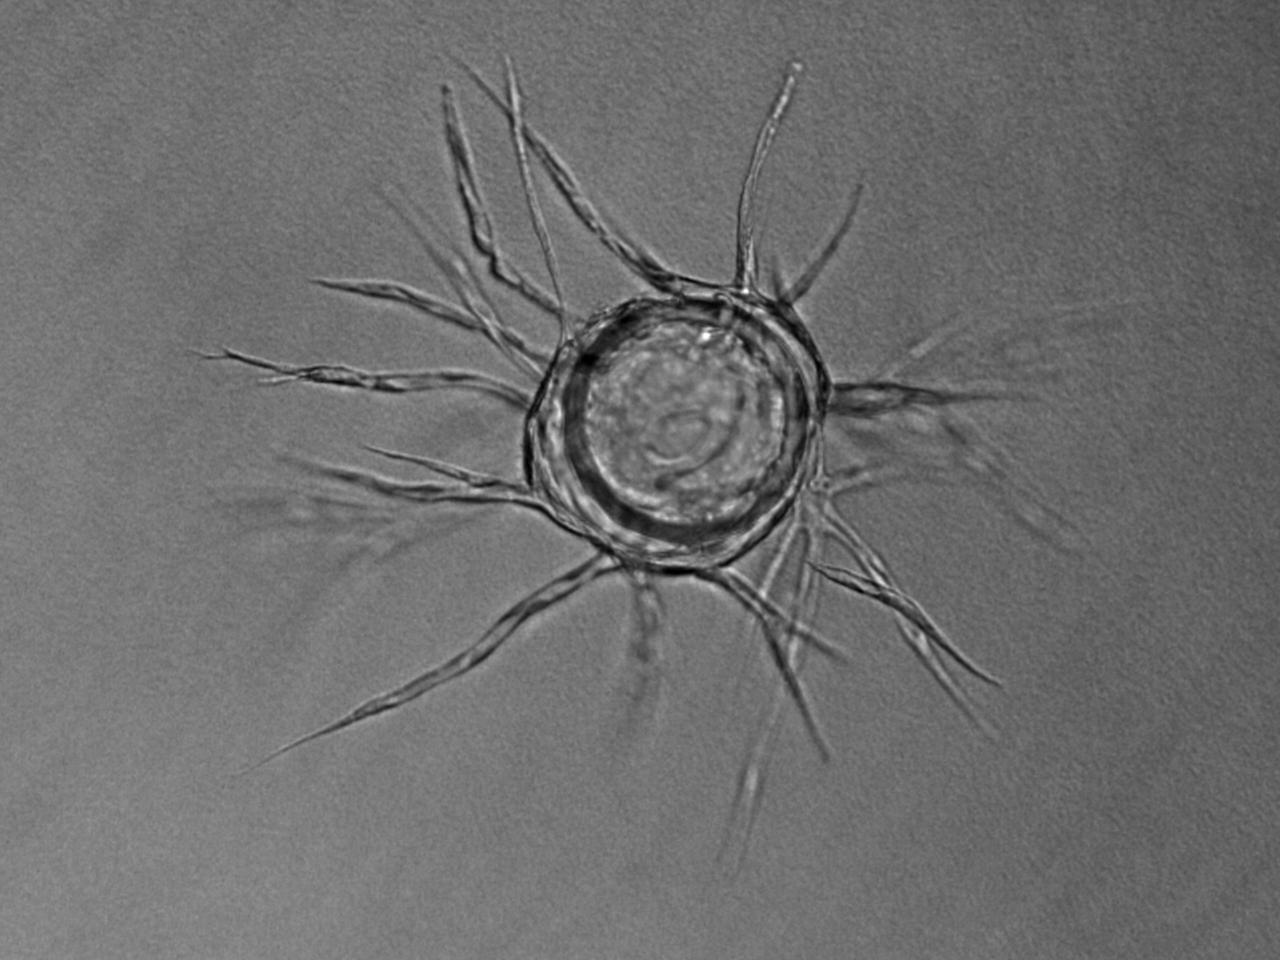
\includegraphics[width=6cm]{images/mono.jpg}
		\caption{Single Bead Image from the Hughes Lab Images}
		\label{fig:monobead}
	\end{figure}

	%% A few definitions
	Components of an image are described as follows. A \emph{bead} refers
	to the Cytodex bead. The \emph{sprouts} are the multicellular
	capillary structures formed by endothelial cells. The \emph{sprout
	count} refers to the number of sprouts per bead. For quantitative
	analysis, the objective of the system is to yield sprout counts that
	are consistent with an expert observer.

	%% How sprout counts were previously acquired
	Previously, the number of sprout counts per bead were measured by manual
	counting on the obtained images. Furthermore, the sprout length was
	ambiguously measured in arbitrary units \cite{nakatsu03}. Our system
	relieves the laborious, manual analysis by quickly automating the detection
	and reliably analyzing of imaged assay features.

	%% Overview of the system
	Our system, the High-Level Sprout Geometry (HLSG) Extractor, is
	designed to detect high-level object and analyze the objects of imaged
	assays. Objects for detection include the Cytodex bead and its
	associated multicellular capillaries. Due to the noise and depth of
	the image, the HLSG Extractor uses structural inpainting to infer
	which sprout segments emerge belong the same sprout. After structural
	inpainting, the HLSG Extractor quantitatively analyzed the images
	using Sholl Analysis to determine the number of primary sprouts and the
	average length for each bead in the imaged assay.

	In addition to the High-Level Sprout Geometry (HLSG) Extractor, a driver
	and report generator are implemented to drive functionality on sample
	images and generate reports on the analyses respectively.

	The following sections will proceed as follows. Section
	\ref{sec:Methodology} will describe an overview of the HLSG feature
	detection and analysis mechanisms. Section \ref{sec:Data Structures}
	will describe the data structures used to represent the HLSG and its
	properties. Section \ref{sec:System Architecture} shows how the system
	is designed for modularity and robustness.
% section Introduction (end)

\section{System Architecture} % (fold)
\label{sec:System Architecture}
	The system requires Python version 2.7x with the SimpleCV package. The
	architecture of the system is based on our methodology for
	quantitatively analyzing \invitro angiogenesis. The system, however,
	incorporates modules for driving batch processes as well as a
	Read-Eval-Print-Loop (REPL) for console interaction. Finally, a module
	incorporated for generating CSV reports of the analysis. The sequence
	diagram for the system components are shown in Figure
	\ref{fig:sysarch}.
	\begin{figure*}[ht!]
		\centering
		\centering
\begin{sequencediagram}
\newinst[1]{client}{User}{}
\newinst[1]{driver}{Driver}{}
\newinst[2]{ex}{Extractors}{}
\newinst[3]{anal}{Sholl Analysis}{}
\newinst[1]{reportgen}{Report Generator}{}

\begin{mess}{client}{images}{driver}{}
	\begin{sdblock}{Main Loop}{}
		\begin{call}{driver}{ExtractHLSGs(img)}{ex}{hlsg}
			\begin{callself}{ex}{ExtractBeads(img)}{beads}
			\end{callself}

			\begin{sdblock}{Sprout Loop}{}
				\begin{callself}{ex}{ExtractSprouts(img, bead)}{sprouts}
				\end{callself}
			\end{sdblock}
		\end{call}

		\begin{call}{driver}{Analyze(hlsg)}{anal}{analysis}
		\end{call}
	\end{sdblock}

	\begin{call}{driver}{GenerateReport(analyses)}{reportgen}{report}
	\end{call}
\end{mess}
\end{sequencediagram}

		\caption{High-Level Architecture}
		\label{fig:sysarch}
	\end{figure*}

	% The REPL module controls the interaction between the user and the
	% system. Commands available in the REPL are shown in Table
	% \ref{tab:commands}.
	% \begin{table}[h!]
	% 	\begin{tabular}{| l | l | p{4cm} |}
	% 		\hline
	% 		\textbf{Command} & \textbf{Output} & \textbf{Description} \\\hline
	% 		extract [file] & HLSG of file & Extracts the HLSG of the given file. \\\hline
	% 		extract [files] & HLSG of files & Extracts the HLSGs of the given files. \\\hline
	% 		exit & Goodbye & Exits the system. \\\hline
	% 	\end{tabular}
	% 	\caption{Commands}
	% 	\label{tab:commands}
	% \end{table}
% section System Architecture (end)


\section{Methodology} % (fold)
\label{sec:Methodology}
	%% PREPROCESSING
	%% Edge Detection for BW Image

	%% BEAD DETECTION
	%% Edge Detection
	%% Hough Transform

	%% NON-BEAD DETECTION
	%% Bead Masking
	%% Edge Detection
	%% Thickening
	%% Thinning
	%% Pruning
	%% Restoration? Consider this as an experiment

	%% SHOLL ANALYSIS
	%% Statistical Analysis

	Our system enables detection of high-level features and quantitative
	analysis of morphometrics which can be decomposed into four stages.
	The first stage is preprocessing: obtain a black and white image such
	that the foreground only contains two objects of interest: beads and
	sprout segments. The second stage is bead detection where the system
	finds the origin and radius of each bead in the image.  The third
	stage is non-bead detection where the system collects all sprout
	segments from the image. Once the sprout segments are collected, the
	system adjusts the sprout segments to reduce noise in the analysis
	stage. The system begins by restoring holes and small gaps within
	sprout segments. Second, spurious arcs and noise are pruned. Finally,
	the resulting image is analyzed through Sholl Analysis which collects
	the number of crossings for a set of concentric circles with a fixed
	origin as the origin of a detected bead.

	% \begin{figure}[htp!]
	% 	\centering
	% 	\subfigure[Sprout Segments]{
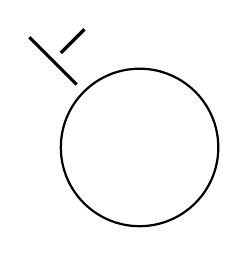
\begin{tikzpicture}
	\node [draw, thick, circle, text centered,  minimum size=2cm] at (0,0) {}; 
	%% BL Sprout
	\draw [very thick] (-0.8,0.8) -- +(-0.6,0.6);
	\draw [very thick] (-1,1.2) -- +(0.3,0.3);
	%\node at (-1.2, -2) {$(d)$};
\end{tikzpicture}
}
\subfigure[Branching]{
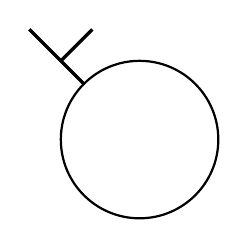
\begin{tikzpicture}
	\node [draw, thick, circle, text centered,  minimum size=2cm] at (0,0) {}; 
	%% TL Sprout
	\draw [very thick] (-0.7,0.7) -- +(-0.7,0.7);
	\draw [very thick] (-1,1) -- +(0.4,0.4);
	%\node at (-1, 2) {$(c)$};
\end{tikzpicture}
}
\subfigure[Junction Point]{
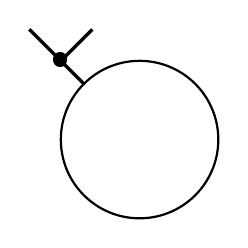
\begin{tikzpicture}
	\node [draw, thick, circle, text centered,  minimum size=2cm] at (0,0) {}; 
	%% TL Sprout
	\draw [very thick] (-0.7,0.7) -- +(-0.7,0.7);
	\draw [very thick] (-1,1) -- +(0.4,0.4);
	\node at (-1,1) {\Large\textbullet};
	%\node at (-1, 2) {$(c)$};
\end{tikzpicture}
}

	% 	\caption{Branching Geometry}
	% 	\label{fig:beadex}
	% \end{figure}

	\subsection{Preprocessing} % (fold)
	\label{sub:Preprocessing}

	In the preprocessing step, the system converts the image into a black
	and white image where white represents the foreground and black
	represents the background. Objects in the foreground are elements of
	interest. Specifically, a foreground object can belong one of three
	higher-order objects: a bead, a sprout segment or noise. Noise is an
	artifact generated from the original image as well as the image
	processing techniques. We use the Canny edge detection algorithm
	\cite{canny86} to obtain the black and white images such the edges
	represent the contours of the elements of interest.
	\begin{figure}[htp!]
		\centering
		\subfigure[Original]{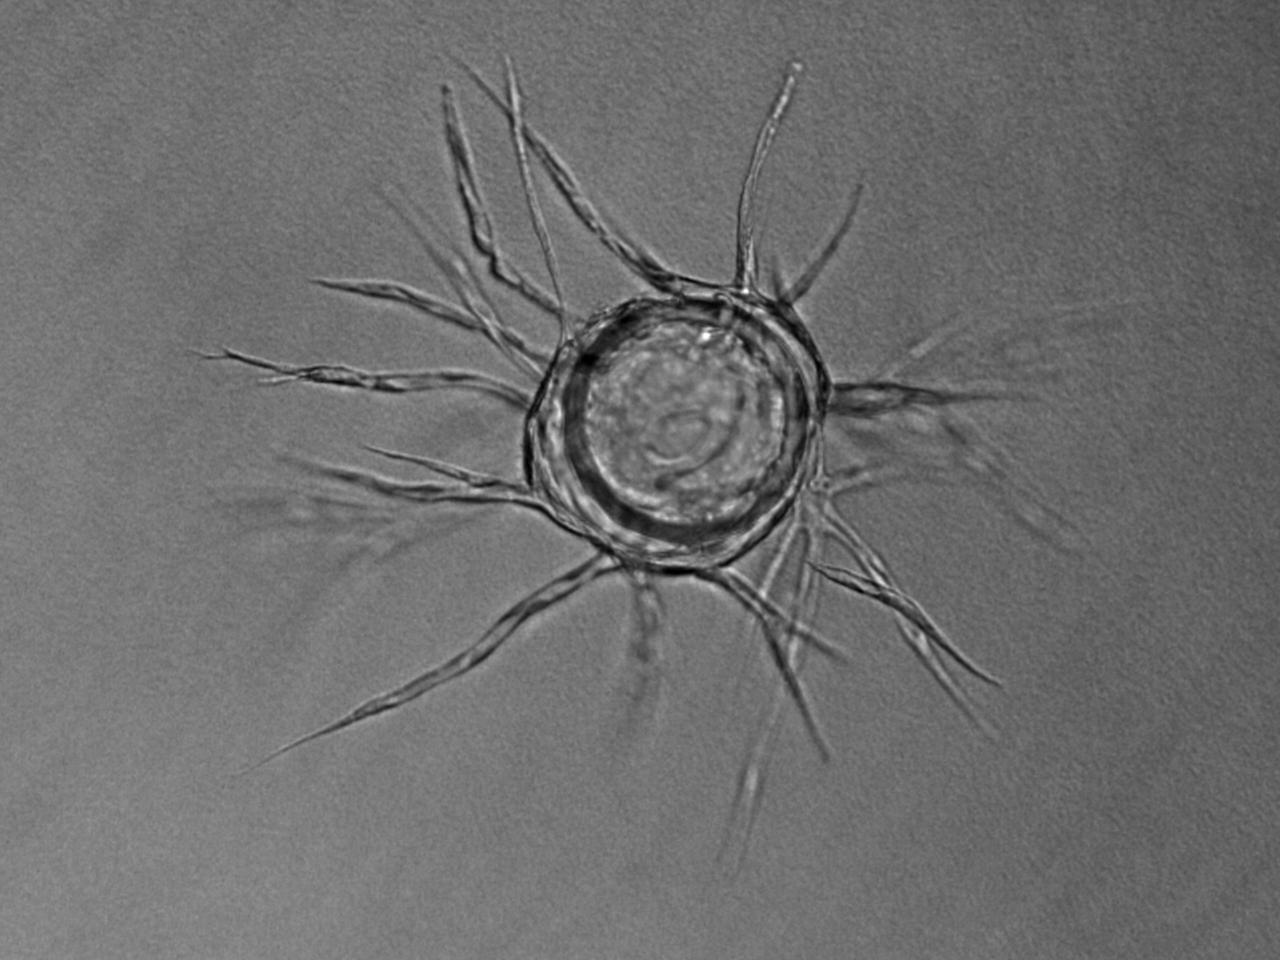
\includegraphics[width=4.1cm]{images/mono.jpg}}
		\subfigure[Edges]{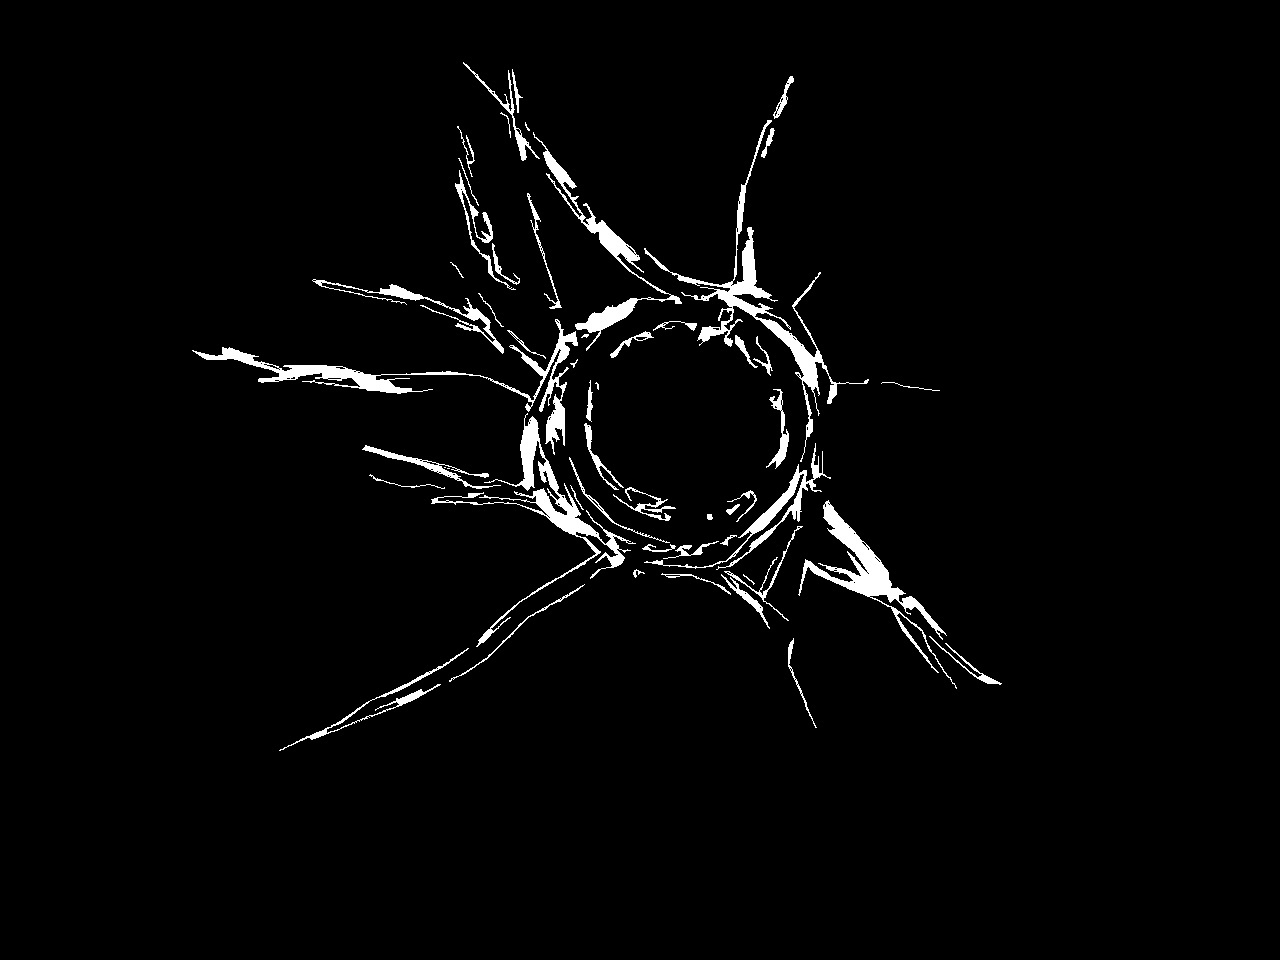
\includegraphics[width=4.1cm]{images/mono_preprocessed.jpg}}
		\caption{Edge Detection Outline}
		\label{fig:beadex}
	\end{figure}
	
	% subsection Preprocessing (end)

	\subsection{Bead Detection} % (fold)
	\label{sub:Bead Extraction}
		Bead detection is a three-step process. To reduce noise, the
		system first smooths the image using a Gaussian blur. Next, the
		system obtains a black and white version of the image through the
		edges of the image using the Canny edge detection algorithm.
		Finally, circles in the image are detected using the circular
		Hough Transform \cite{yuen89}. The circles detected correspond to
		the beads in the imaged assay. It follows that the origin and
		radius of the bead are obtained.
		\begin{figure}[htp!]
			\centering
			% \subfigure[Original]{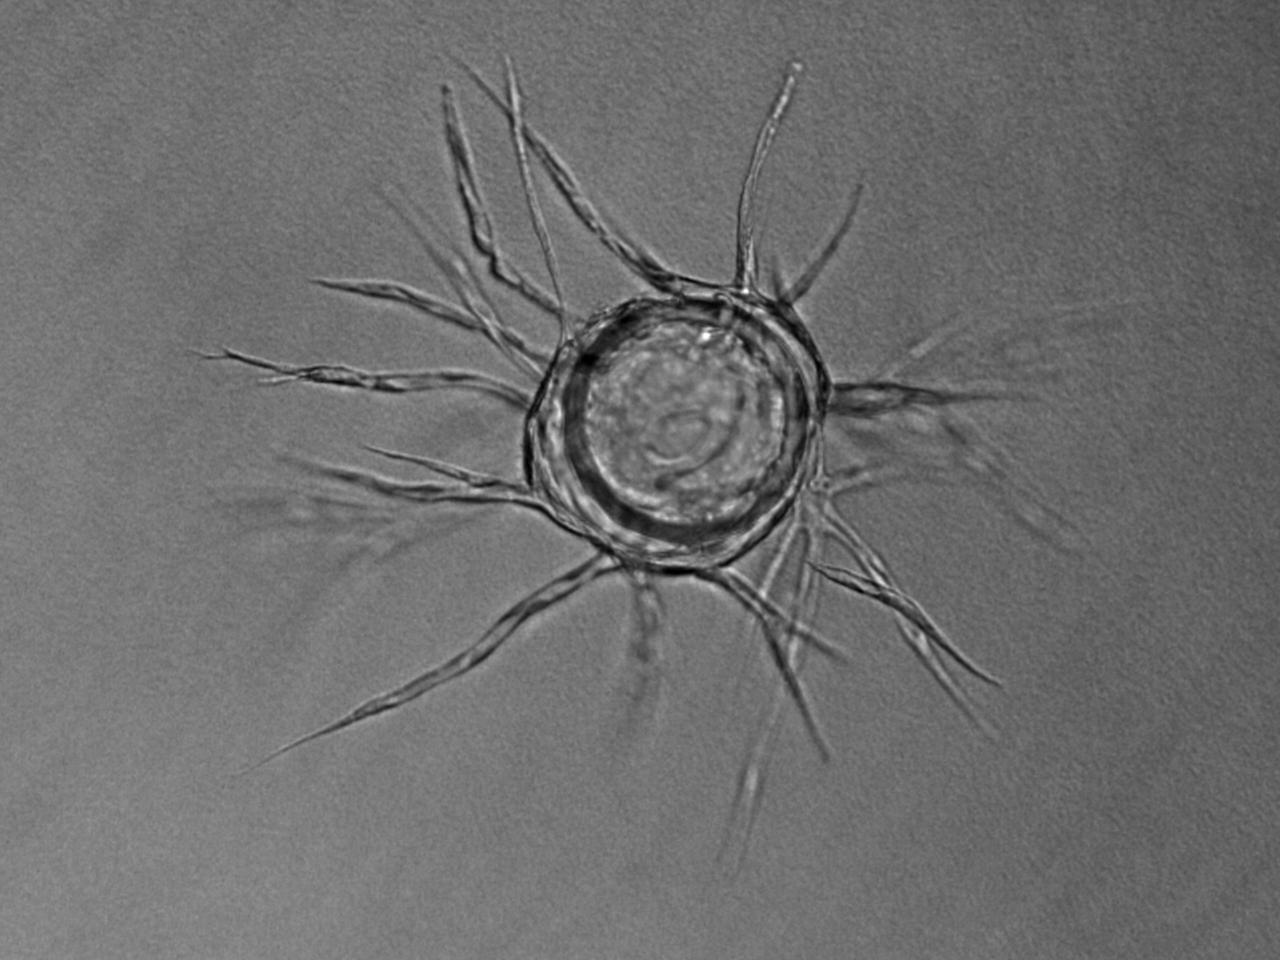
\includegraphics[width=4.1cm]{images/mono.jpg}}
			\subfigure[Edges]{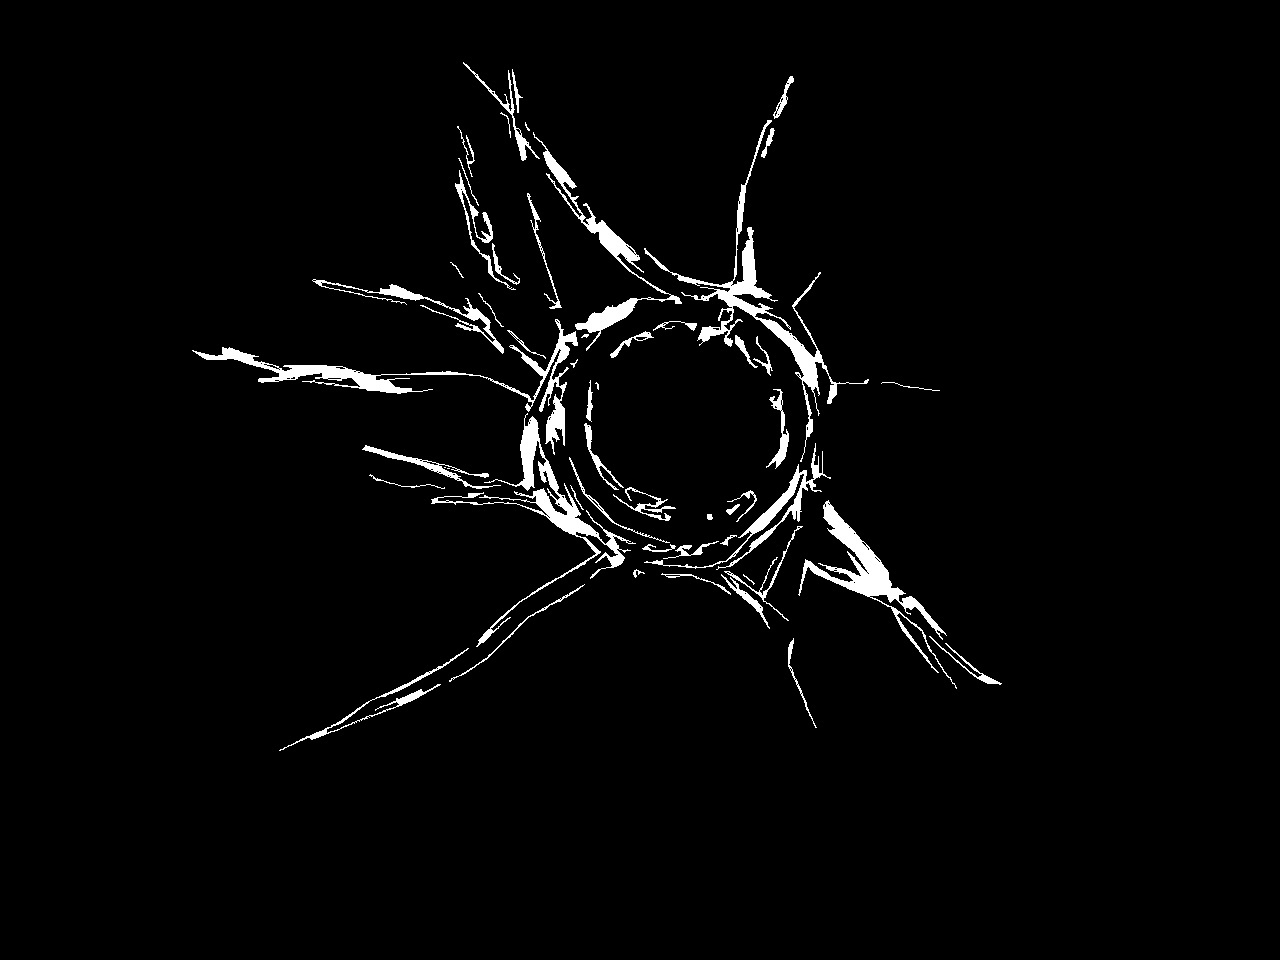
\includegraphics[width=4.1cm]{images/mono_preprocessed.jpg}}
			\subfigure[Bead Detection]{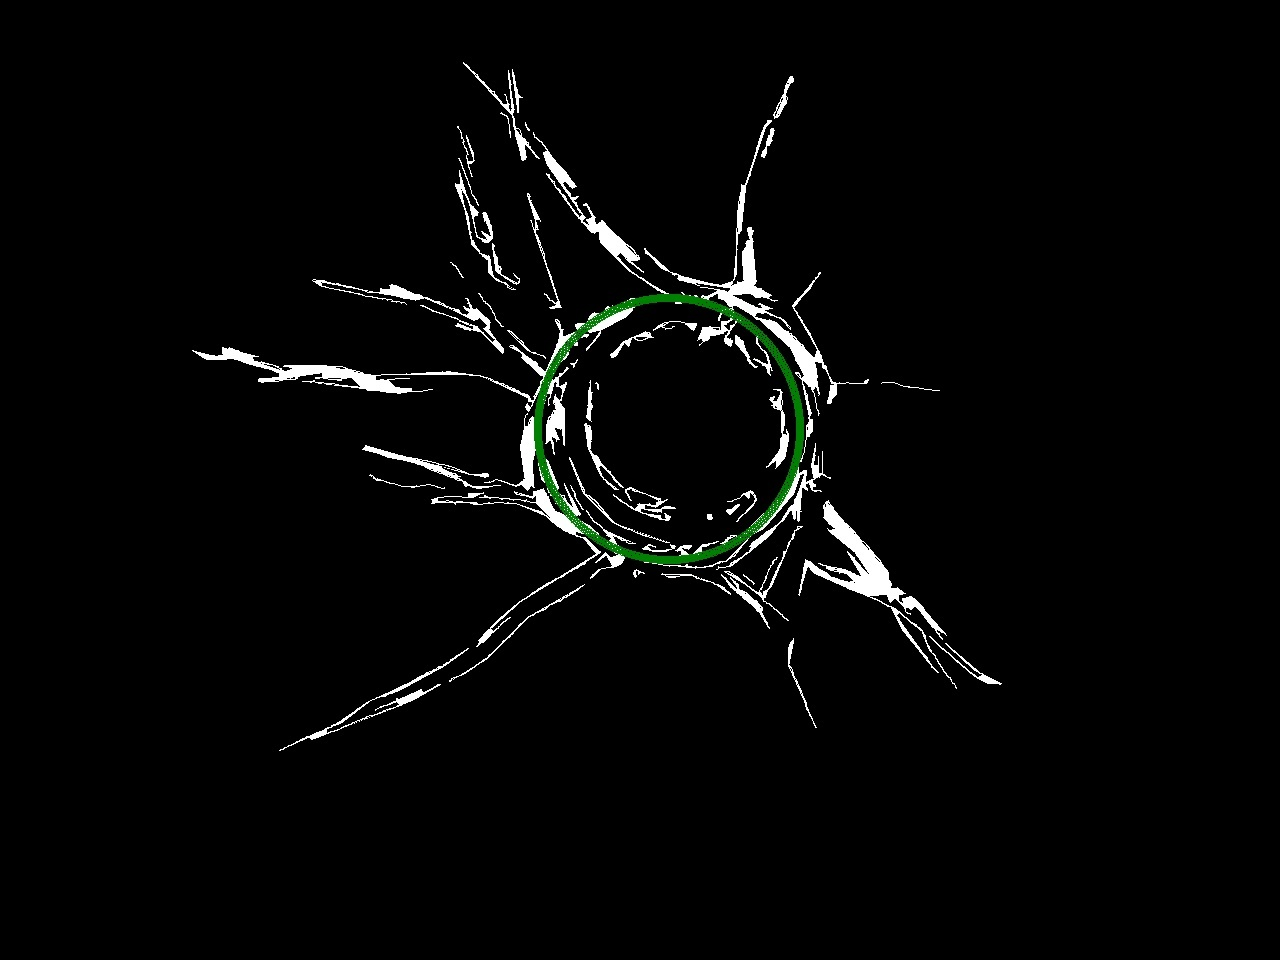
\includegraphics[width=4.1cm]{images/mono_found_circle.jpg}}
			\caption{Bead Detection Outline}
			\label{fig:beadex}
		\end{figure}

		In order to avoid false bead detections, we enforce that the
		minimum distance between the origin of every pair of detected
		circles be four times the average bead radius while preferring
		beads with the more votes in the accumulator i.e.  each detected
		bead should at least be a bead apart. We ignore the degenerate
		case in which two or more beads are within the distance constraint
		because associating sprouts to beads becomes inaccurate.
	% subsection Bead Extraction (end)

	\subsection{Non-Bead (Sprout) Detection} % (fold)
	\label{sub:Sprout Extraction}
		%% Thickening
		%% Thinning
		%% Pruning
		The system begins by obtaining a black and white image from the
		grayscale imaged assay. Since the edges of the images represent
		the contours of beads, sprouts and noise, we mask the detected
		beads such that only the sprout and noise contours remain. The noise
		is reduced in the sprout restoration phase.
		\begin{figure}[htp!]
			\centering
			\subfigure[Original]{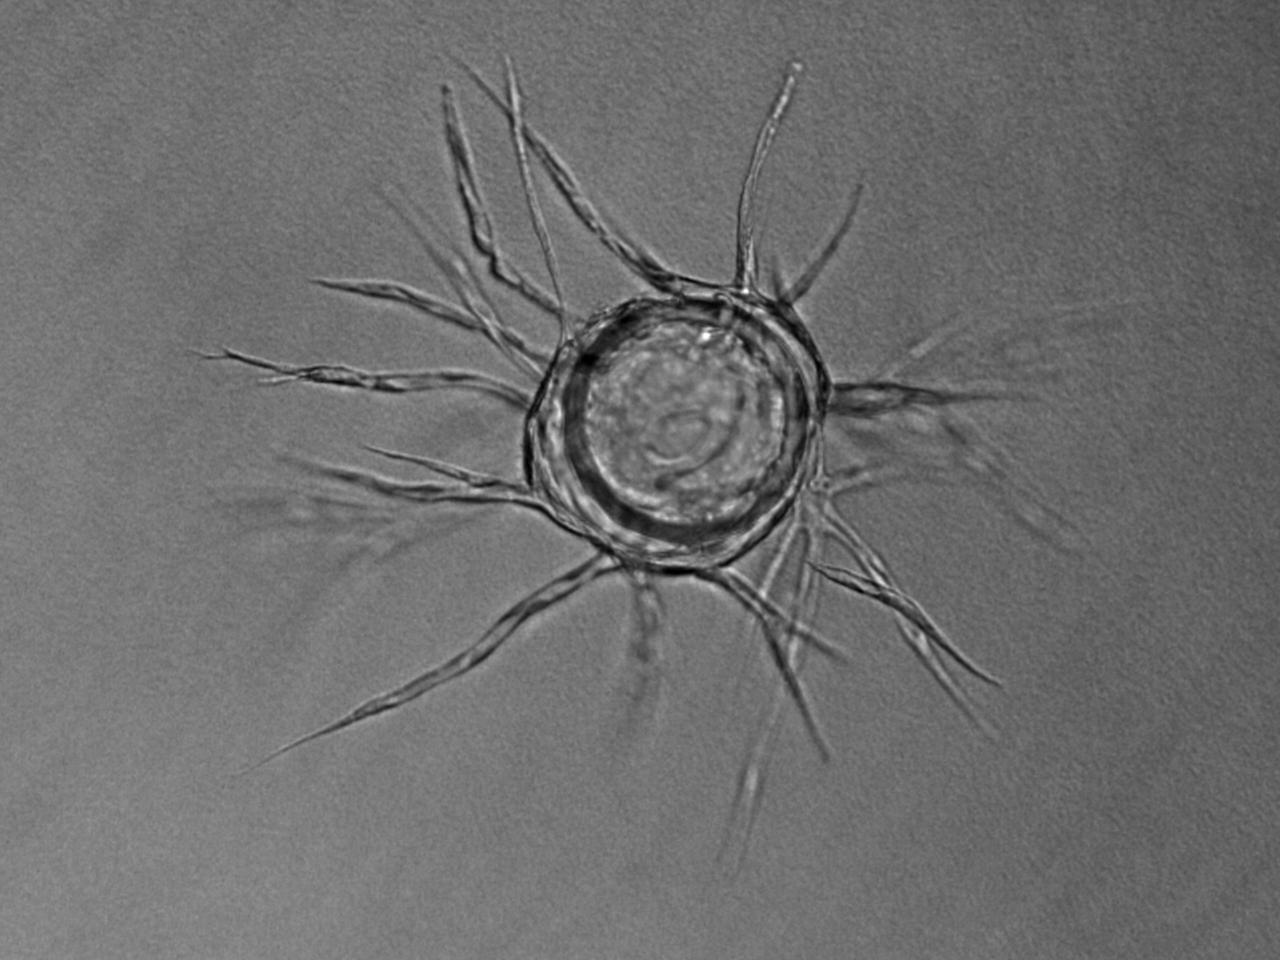
\includegraphics[width=4.1cm]{images/mono.jpg}}
			\subfigure[Edges]{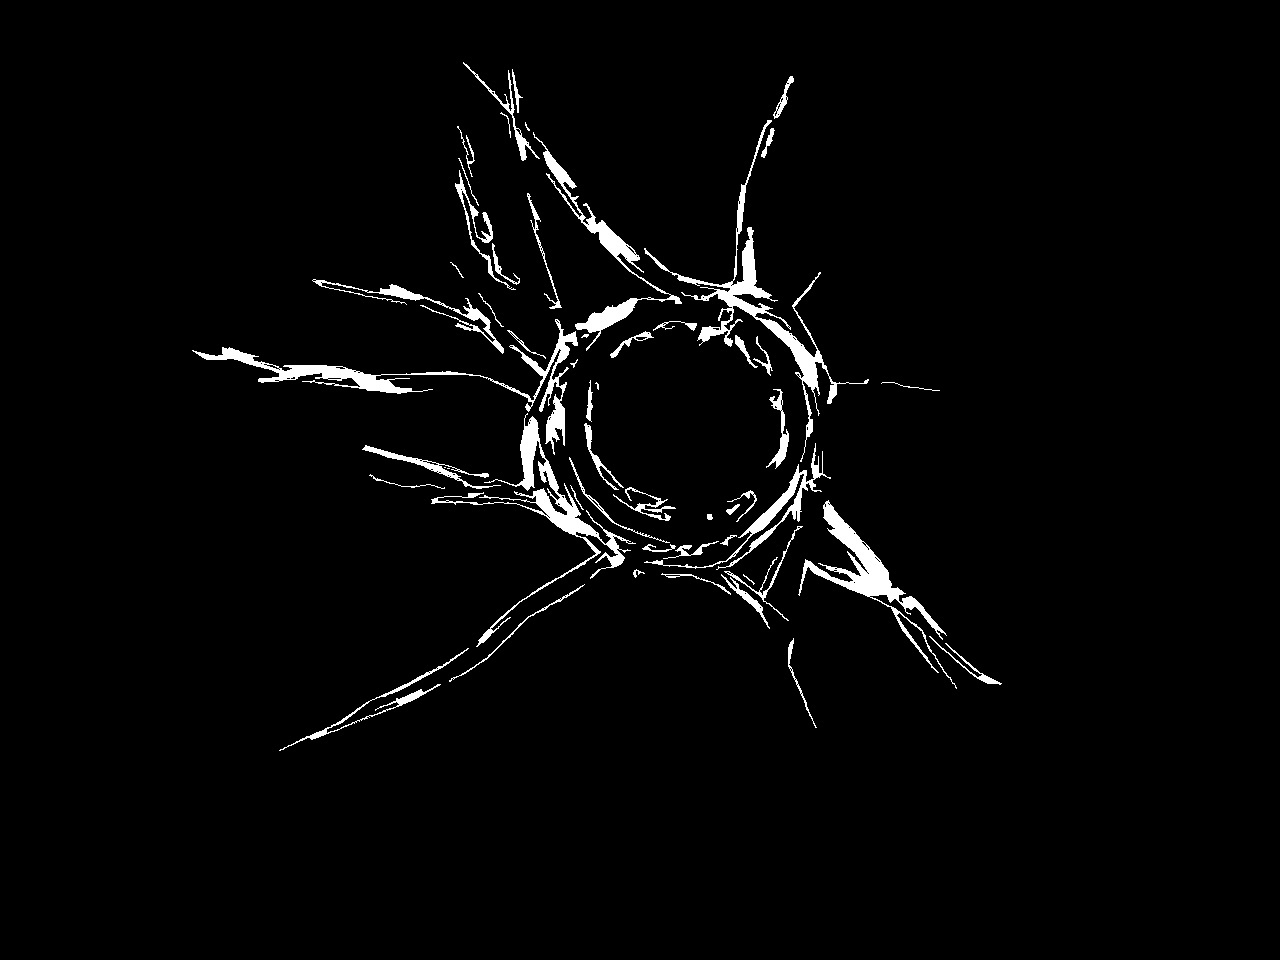
\includegraphics[width=4.1cm]{images/mono_preprocessed.jpg}}
			\caption{Edge Detection Outline}
			\label{fig:beadex}
		\end{figure}

		Since the borders of the sprouts are detected as edges, they may
		appear to be distinctly segmented objects. We call such objects
		\emph{sprout segments}. Subsequently, it is necessary that the
		system links the sprout segments to reconstruct the original
		sprout.

		%% Thickening and thinning
		The system approaches the reconstruction by first thickening the
		sprout segments until the lumen disappears. Next, the thickened
		structure is is skeletonized by thinning. Since the skeleton
		represents the fundamental morphology of the structure, and
		approximate centerline for each of the sprouts are generated.
		\begin{figure}[htp!]
			\centering
			\subfigure[Thickening]{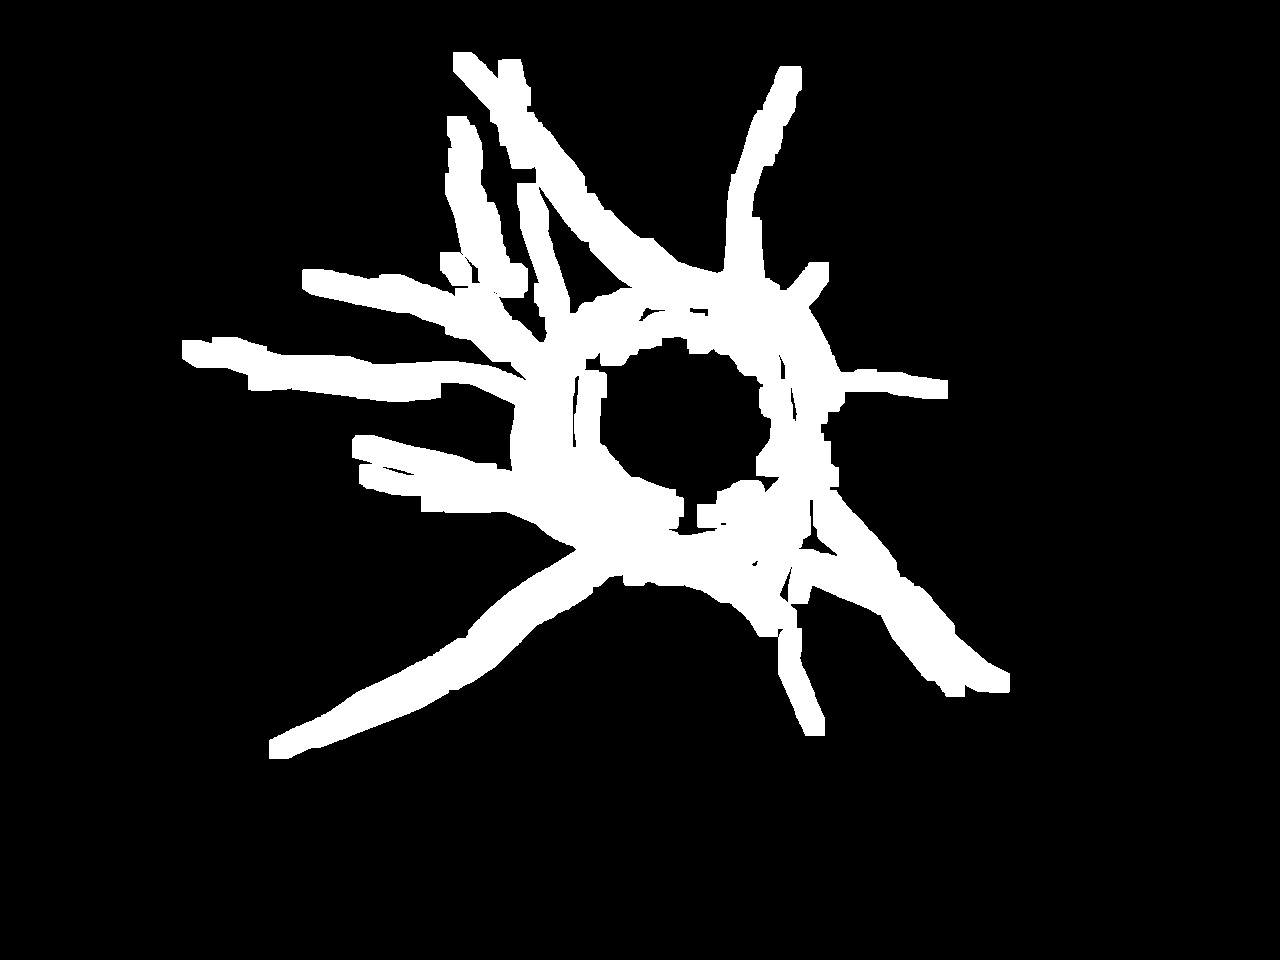
\includegraphics[width=4.1cm]{images/mono_dilated.jpg}}
			\subfigure[Thinning and Pruning]{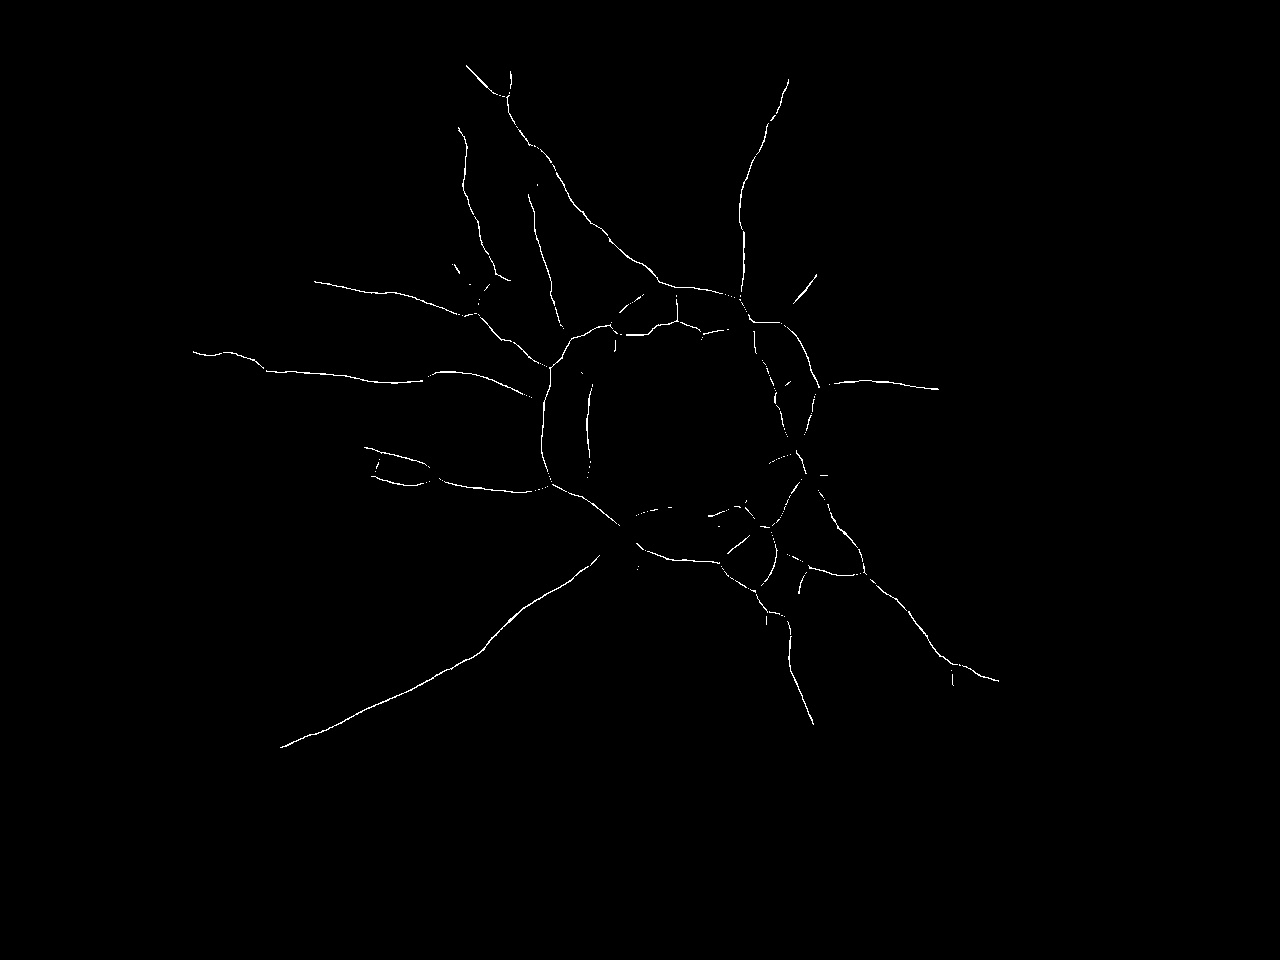
\includegraphics[width=4.1cm]{images/mono_skeletonized.jpg}}
			\caption{Sprout Detection Outline without Bead Masks}
			\label{fig:sproutex}
		\end{figure}
		We now utilize the disjoint centerlines as sprout segments.
		
		\subsubsection{Sprout Segment Connectivity} % (fold)
		\label{ssub:Sprout Segment Connectivity}
			Due to the discontinuity of sprouts in the assay, we begin by
			collecting all sprout segments and represent them as line
			segments. We distinguish the end points of each line segment
			as either an inner point or outer point. The inner point, $I$,
			is the end point on the line segment such that it is closer to
			the origin of the line segment's closest bead. The outer
			point, $O$, is the end point on the line segment such that it
			is farther from the origin of the line segment's closest bead.

			To determine which line segments belong to the same sprout, we
			use Euclidean distance between their inner and outer points
			enforced by the constraint that the end point must be closer
			to the origin of its closest bead than the target start point.
			For example, two line segments are part of the same sprout if
			the distance between the start and end points are within a
			specified distance parameter, $d$.

			Once the sprouts segments have been connected, we refer to the
			connected structures as sprouts.
		% subsubsection Sprout Segment Connectivity (end)

		\subsubsection{Sprout Restoration} % (fold)
		\label{sub:Sprout Restoration}
			In this phase, there are two primary sources of degradation
			observed. First, noise is still in the foreground after
			sprouts segments are connected. Second, holes may exist in
			the morphology of the sprouts after thickening and thinning
			the structures. We describe our methods for resolving each
			problem independently.

			Noise in the image can be described in two common forms:
			isolated points and spurious arcs. Isolated points refer to
			the small objects detected in the foreground that have no
			apparent relation to sprout segments. Spurious arcs are
			auxiliary stubs that are generated from skeletonization. To
			remove the noise from the black and white image, we apply
			several hit-and-miss transformation that masks isolated points
			and spurious arcs. Hence, only the sprout segments remain.
			\begin{figure}[htp]
				\[
					\left(\begin{matrix}
						-1 & -1 & -1 & -1 & -1 \\
						-1 & 0 & 0 & 0 & -1 \\
						-1 & 0 & 1 & 0 & -1 \\
						-1 & 0 & 0 & 0 & -1 \\
						-1 & -1 & -1 & -1 & -1 \\
					\end{matrix} \right)
				\]
				\caption{Hit-and-Miss Transformation Kernel for Isolated
				Points where $1$ represents foreground, $-1$ represents
				background and $0$ can be either}
			\end{figure}

			In contrast with noise, holes are points that can be found
			within foreground structures that should have been detected as
			foreground. These holes are primarily artifacts of the Canny
			edge-detection algorithm since the contours of a capillary
			encompass the lumen which is detected as background. By the
			morphology of these structures, we simply find the contours
			which enclose small holes and perform inpainting.
		% subsubsection Sprout Restoration (end)

	% subsection Sprout Extraction (end)

	\subsection{Sholl Analysis} % (fold)
	\label{sub:Sholl Analysis}
		Sholl Analysis is a quantitative method for quantitatively
		analyzing morphological characteristics of neurons \cite{sholl53}.
		We use Sholl Analysis because the morphology of our imaged assays
		closely resembles neuron images after our preprocessing steps.

		Briefly, Sholl Analysis consists of counting the number of
		foreground to background crossings given concentric circles of a
		centered at the origin of a bead. The algorithm can then be
		decomposed into initialization, iteration and final stages. For
		the intialization, we select a bead, $B$. Next, let the initial
		circle radius, $r_{\min}$, be slightly larger than the detected
		radius of the bead and let the maximum radius, $r_{\max}$, be the
		minimum distance from the origin of the detected bead to either of
		the four image borders. For each radius, $r \in [r_{\min},
		r_{\max}]$, we we define the number of crossings as $N(r)$. For further analysis,
		we define the critical value, $\text{CV}(N)$, as the radius at which
		the maximum number of crossings occur. See \ref{app:Sholl
		Analysis} for the pseudo code using an optimized Bresenham Circle
		Algorithm.
		
		For posterior analysis, we define longest increasing subsequence
		(LIS) of $N(r)$ as $\text{LIS}(N)$ with the domain constrained
		between $[r_{\min}, \text{CV}(N)]$. The longest decreasing
		subsequence (LDS), $\text{LDS}(N)$ is defined similarly with the
		domain constrained to $[\text{CV}(N), r_{\max}]$. The LIS and LDS
		guarantee that we have strictly increasing counts to ignore gaps
		as noise.

		From the number of crossings, we determine the sprout counts and
		average length. The sprout counts, $c_N$, are determined by a
		median of the $\text{LIS}(r)$. To determine the average length,
		$l_N$, we define a proecdure. First, we define by the radius at
		which $\text{LDS}(N)$ has a value of $1$ as $l_{\max}$ and we
		define the radius at which $\text{LDS}(N)$ has a value of
		$c_N$ as $l_{\min}$. Then, we calculate $l_N$ as the average
		of $l_{\max}$ and $l_{\min}$.
	% subsection Sholl Analysis (end)
% section Methodology (end)

% \section{Data Structures} % (fold)
% \label{sec:Data Structures}
% 	The following data structures are used to implement the HLSG Extractor.
% 	\begin{figure}[!ht]
% 		\centering
% 		\begin{tikzpicture}[scale=0.5]
\umlclass[x=0,y=0]{BeadFeature}{
	+ center : (uint, uint) \\
	+ radius : uint \\
	}{}
\umlclass[x=4.5,y=0]{SproutFeature}{
	+ centroid : (uint, uint) \\
	+ length : uint \\
	+ width : uint \\
	}{}
\umlclass[x=4.5,y=-3]{RadialSegment}{
	+ inner : (uint, uint) \\
	+ outer : (uint, uint) \\
	+ blob : Blob
	}{}
%% Relations
\umlaggreg{BeadFeature}{SproutFeature}
\umluniaggreg{SproutFeature}{RadialSegment}
\end{tikzpicture}

% 		\caption{HLSG Extractor Features Class Diagram}
% 		\label{fig:classdiag}
% 	\end{figure}
% 
% 	\subsection{Bead Feature} % (fold)
% 	\label{sub:Bead Feature}
% 		A bead feature is an abstraction of the Cytodex bead coated with
% 		endothelial cells in the assay. The geometry of the bead is intuitively
% 		circular; subsequently the geometry can is described by the descriptor
% 		in Figure \ref{fig:classdiag}.
% 	% subsection Bead Feature (end)
% 
% 	\subsection{Sprout Feature} % (fold)
% 	\label{sub:Sprout Feature}
% 		A sprout feature is an abstraction of the blood vessels that develop
% 		through angiogenesis from the designed bead. Subsequently, sprout
% 		feature extraction is dependent upon bead descriptors. The sprout is
% 		actually comprised of a set of pixel segments because of the
% 		possibility that a sprout is disconnected.
% 	% subsection Sprout Feature (end)
% 
% 	\subsection{Radial Line Segment} % (fold)
% 	\label{sub:Radial Line Segment}
% 		Due to the disconnectivity of sprouts, individual sprout segments
% 		are represented by a radially defined line segment. That is, we
% 		distinguish the end points from its radial distance from the origin
% 		of its corresponding bead. Given a line segment, we say that and
% 		end point is the \emph{inner point} if it is radially closer than
% 		its complementary end point; otherwise, we call the end point the
% 		\emph{outer point}.
% 
% 		In addition to the distinguishable end points, a radial line
% 		segment is a line fit onto a corresponding blob of pixels which can
% 		be considered a sprout segment.
% 	% subsection Radial Line Segment (end)
% 
% 	\subsection{Driver} % (fold)
% 	\label{sub:Driver}
% 		The Driver is responsible for parsing input from the user and emulating
% 		the encoded actions as functions of the HLSG Extractor. That is, the
% 		Driver acts similar to a REPL (Read-Eval-Print-Loop) that reads input
% 		from the user, evaluates the input and prints the corresponding output
% 		in a loop. The set of commands available to the user is outlined Table
% 		\ref{tab:commands}.
% 	% subsection Driver (end)
% % section Data Structures (end)

\section{Results} % (fold)
\label{sec:Results}
	The results of our sprout counts show a standard error of $1.7$ when
	compared manual sprout counts of an expert observer (see Table
	\ref{tab:resultcomp}). In the table, the expert observer sprout counts
	include only sprouts which are declared to be in-focus.

	\begin{table}[htp]
		\centering
		\begin{tabular}{| l | l | l |}
			\hline
			\textbf{Treatment} & \textbf{Human Counts} & \textbf{HLSG Counts} \\\hline
			10k 1 Day 7 & 7  & 10 \\\hline
			10k 5 Day 7 & 10 &  10 \\\hline
			1k 2 Day 7 & 11 & 9 \\\hline
			1k 3 Day 7 & 14 & 14 \\\hline
			20k 1 Day 7 & 15 & 10 \\\hline
			20k 2 Day 7 & 15 & 12 \\\hline
			20k 3 Day 7 & 6 & 8 \\\hline
			20k 5 Day 7 & 9 & 10 \\\hline
			Ang1 100 ng/ml 3 Day 7 & 7 & 9 \\\hline
			Ang1 100 ng/ml 5 Day 7 & 9 & 12 \\\hline
			Ang1 250 ng/ml 1 Day 7 & 8 & 7\\\hline
			Control 1 Day 7 & 10 & 12 \\\hline
			Control 2 Day 7 & 12 & 13 \\\hline
			Control 4 Day 7 & 8 & 8 \\\hline
			Control 5 Day 7 & 7 & 9 \\\hline
		\end{tabular}
		\caption{Expert Observer vs. HLSG Sprout Counts}
		\label{tab:resultcomp}
	\end{table}

	The average lengths have also been obtained with arbitrary units;
	however, there currently exists no average length data from an expert
	observer for comparison.
% section Results (end)

\section{Discussion} % (fold)
\label{sec:Discussion}
	The sprout count results demonstrate consistency with human observers
	for in focus sprouts. Our HLSG Extractor, however, also shows a
	consistent pattern in overestimating the number of sprouts
	declared to be in-focus by an expert observer. This occurs because
	our system may also capture sprouts that were declared to be
	out-of-focus by an expert observer. The preprocessing phase of our
	methodology uses edge detection to determine which sprouts to
	count whereas an expert observer may utilize other features beyond
	a discernable cell wall.

	Furthermore, we speculate that sprouts crossings and sprout
	discontinuities are the greatest sources of error in sprout counts.
	Sprout crossings are defined to be the occurrence of two overlapping
	sprouts. A method of effectively distinguishing sprout branching from
	sprout crossings is still an open problem. Additionally, more
	effective sprout restoration methods could improve the accuracy of
	Sholl Analysis.
% section Discussion (end)

\section{Conclusions} % (fold)
\label{sec:Conclusions}
	Automated image analysis methods are necessary for the assessment of
	pro-angiogenic and anti-angiogenic agents in an \invitro angiogenesis
	assay. Unfortunately, the methodology of contemporary software is
	insufficient for our data set. Manual methods are also laborious and
	vulnerable to observer bias.

	To overcome these shortcomings, we have designed an optimized image
	analysis method for quantitatively analyzing \invitro angiogenesis
	assays containing HUVEC. The system, HLSG Extractor, obtains sprout
	counts that are consistent with the accuracy of an expert observer. In
	addition to sprout counts, the average length of the sprouts per bead
	have are also obtained. With the versatility of Sholl Analysis,
	several other morphometrics may become available using further
	statistical methods.

	%% Future work
	Potential adjustments to the system may include new implementations
	and different approaches to the phases of the optimized methodology.
	For example, given the sprout counts of the bead of an imaged assay,
	we may reduce the noise from discontinuous sprouts further by a
	piecewise constant approximation of the sprout counts. Subsequently,
	methods of integration may be unnecessary. 

	%% Summary
	Cumulatively, the HLSG Extractor has proven to be a consistent, robust
	and automated image analysis system of \invitro angiogenesis
	morphology.
% section Conclusions (end)

\section{Acknowledgements} % (fold)
\label{sec:Acknowledgements}
	We would like to thank Dr. Ernie Esser and Anna Konstorum from the
	Department of Mathematics, University of California, Irvine, for
	valuable commentary and guidance throughout the research process. We
	would also like to acknowledge the laboratory of Dr. Chris Hughes in
	the Department of Molecular Biology \& Biochemistry at UC Irvine for
	making available the image sets of their fibrin gel bead sprouting
	assays. This research was funded by the National Science Foundation
	(NSF) DMS-0928427.
% section Acknowledgements (end)

\bibliography{prelim}
\bibliographystyle{plain}

\appendix
\section{Pseudo Code} % (fold)
\label{sec:Pseudo Code}
	This section outlines the pseudo code for Sholl Analysis by using an
	optimized Bresenham Circle Algorithm for circular point generation.

	\subsection{Sholl Analysis} % (fold)
	\label{app:Sholl Analysis}
	Sholl Analysis counts the number of crossings for a set of concentric
	circles from an initially defined radius to a maximally defined
	radius. See Algorithm 1 for our precise
	implementation.
		\begin{algorithm}[ht!]
			\caption{Sholl Analysis}
			\begin{algorithmic}
				\Procedure{ShollAnalysis}{img, origin, radius}
					\State $r_{\min} \gets$ radius
					\State $r_{\max} \gets$ $\min\left\{\text{origin.x, img.width - origin.x}\right\}$
					\State $r_{\max} \gets$ $\min\left\{r_{\max}, \text{ origin.y, img.height - origin.y}\right\}$
					\State crossings $\gets$ empty dictionary
					\ForAll{$r \in [r_{\min}, r_{\max}]$}
						\State crossings[$r$] $\gets$ \Call{CountCrossings}{img, origin, $r$}
					\EndFor
					\State \Return crossings
				\EndProcedure
			\end{algorithmic}
			\begin{algorithmic}
				\Procedure{CountCrossings}{img, origin, radius}
					\State crossings $\gets$ 0
					\ForAll{pixel $\in$ \Call{BresenhamCircle}{origin, radius}}
						\If{crossing detected at pixel}
							\State crossings $\gets$ crossings + 1
						\EndIf
					\EndFor
					\State \Return crossings
				\EndProcedure
			\end{algorithmic}
		\end{algorithm}
	% subsection Sholl Analysis (end)

	\subsection{Ordered Bresenham Circle Algorithm} % (fold)
	\label{app:Ordered Bresenham Circle Algorithm}
		Bresenham's circle algorithm is frequently used to determine which
		pixels should be selected to draw a circle. algorithm utilizes
		symmetry of a circle in order to reduce the running time by a
		factor of eight \cite{bresenham77}. For our application with Sholl
		Analysis, the algorithm must return the points as an ordered set
		which is defined to be counterclockwise starting from the positive
		x-axis.

		The algorithm calculates points for all eight octants simultaneously.
		The octants are labeled with integers starting with zero. We label the
		octants from starting from the x-positive axis in the counterclockwise
		direction. The labels can be seen in figure \ref{fig:eightsymmetry}.
		\begin{figure}[htp]
			\centering
			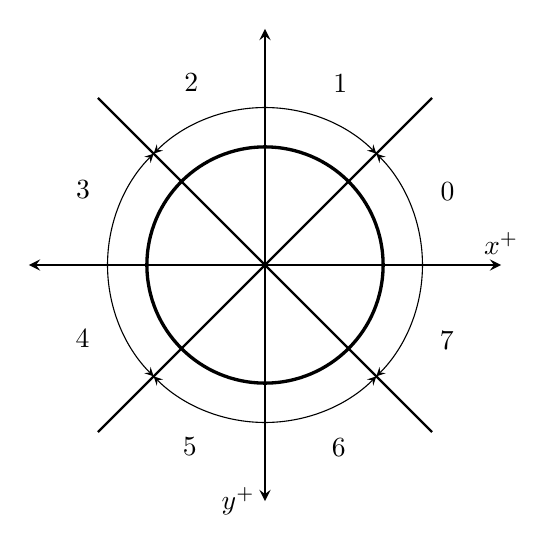
\begin{tikzpicture}[>=stealth]
	\draw [very thick] (0,0) circle (1.5);

	%% Coordinate axes
	\draw [<->,thick] (-3,0) -- (3,0) node [above] {$x^+$};
	\draw [<->,thick] (0,3) -- (0,-3) node [left] {$y^+$};

	%% Diagonals
	\draw [thick] (0,0) +(45:-3) -- (45:3);
	\draw [thick] (0,0) +(135:-3) -- (135:3);

	%% Even arcs
	\foreach \x in {0,1,2,3} {
		\pgfmathmultiply{\x}{90}
		\pgfmathtruncatemacro{\alpha}{\pgfmathresult}
		\draw [->] (0,0) +(0+\alpha:2cm) arc (0+\alpha:45+\alpha:2cm);
		\pgfmathmultiply{\x}{2}
		\pgfmathtruncatemacro{\arclabel}{\pgfmathresult}
		\path (0,0) +(22+\alpha:2.5cm) node {$\arclabel$};
	}

	%% Odd arcs
	\foreach \x in {0,1,2,3} {
		\pgfmathmultiply{\x}{90}
		\pgfmathtruncatemacro{\alpha}{\pgfmathresult}
		\draw [->] (0,0) +(90+\alpha:2cm) arc (90+\alpha:90+\alpha-45:2cm);
		\pgfmathparse{2*\x+1}
		\pgfmathtruncatemacro{\arclabel}{\pgfmathresult}
		\path (0,0) +(67.5+\alpha:2.5cm) node {$\arclabel$};
	}
\end{tikzpicture}

			\caption{Octants in the Eight-Way Symmetry of a Circle}
			\label{fig:eightsymmetry}
		\end{figure}
		Because it is necessary that the points are ordered
		counterclockwise from the positive x-axis, we modify the
		algorithm. The algorithm calculates the points from ordered
		clockwise or counterclockwise from the closest coordinate axis.
		Hence, we reverse the points calculated for every odd octant and
		then concatenate their data points.

		\begin{algorithm}[htp!]
			\caption{Ordered Bresenham Circle Algorithm}
			\begin{algorithmic}
				\Ensure{points returned are ordered counterclockwise from the positive x-axis}
				\Procedure{BresenhamCircle}{origin, radius}
					\State $x \gets$ radius
					\State $y \gets 0$
					\State $r_{\text{error}} \gets 1 - x$
					\State octants $\gets$ empty array
					\While{$x \geq y$}
						\State octants[0] $\Leftarrow$ ($x$ + origin.x, $-y$ + origin.y)
						\State octants[1] $\Leftarrow$ ($y$ + origin.x, $-x$ + origin.y)
						\State octants[2] $\Leftarrow$ ($-y$ + origin.x, $-x$ + origin.y)
						\State octants[3] $\Leftarrow$ ($-x$ + origin.x, $-y$ + origin.y)
						\State octants[4] $\Leftarrow$ ($-x$ + origin.x, $y$ + origin.y)
						\State octants[5] $\Leftarrow$ ($-y$ + origin.x, $x$ + origin.y)
						\State octants[6] $\Leftarrow$ ($y$ + origin.x, $x$ origin.y)
						\State octants[7] $\Leftarrow$ ($x$ + origin.x, $y$ origin.y)
						\State $y \gets y + 1$
						\If{$r_{\text{error}} < 0$}
							\State $r_{\text{error}} \gets r_{\text{error}} + 2y + 1$
						\Else
							\State $x \gets x - 1$
							\State $r_{\text{error}} \gets r_{\text{error}} + 2(y - x + 1)$
						\EndIf
					\EndWhile
					\State points $\gets$ []
					\ForAll{octant $\in$ octants}
						\If{octant is odd}
							\State reverse the octant
						\EndIf
						\ForAll{point $\in$ octant}
							\State points $\Leftarrow$ point
						\EndFor
					\EndFor
					\State \Return points
				\EndProcedure
			\end{algorithmic}
		\end{algorithm}

	% subsection Ordered Bresenham Circle Algorithm (end)
% section Pseudo Code (end)

\end{document}
